\section{Proposed Timeline}

You can use a Gantt chart to visually represent the timeline. Common tasks are listed below; however, you have full freedom to adjust these tasks according to your study. When drawing the Gantt chart, make sure to pin the points where you achieve the objectives.
 
\begin{itemize}
	\item Proposal Writing \& Approval
	\item Literature Review
	\item Dataset Collection or Preprocessing
	\item Model/Framework Development
	\item Evaluation \& Testing
	\item Analysis \& Discussion
	\item Documentation	
\end{itemize}

You can use the time period from this semester to the second semester of Level 400, since you have started your research work in this semester. 

	\begin{figure}[htbp]
		\centering
		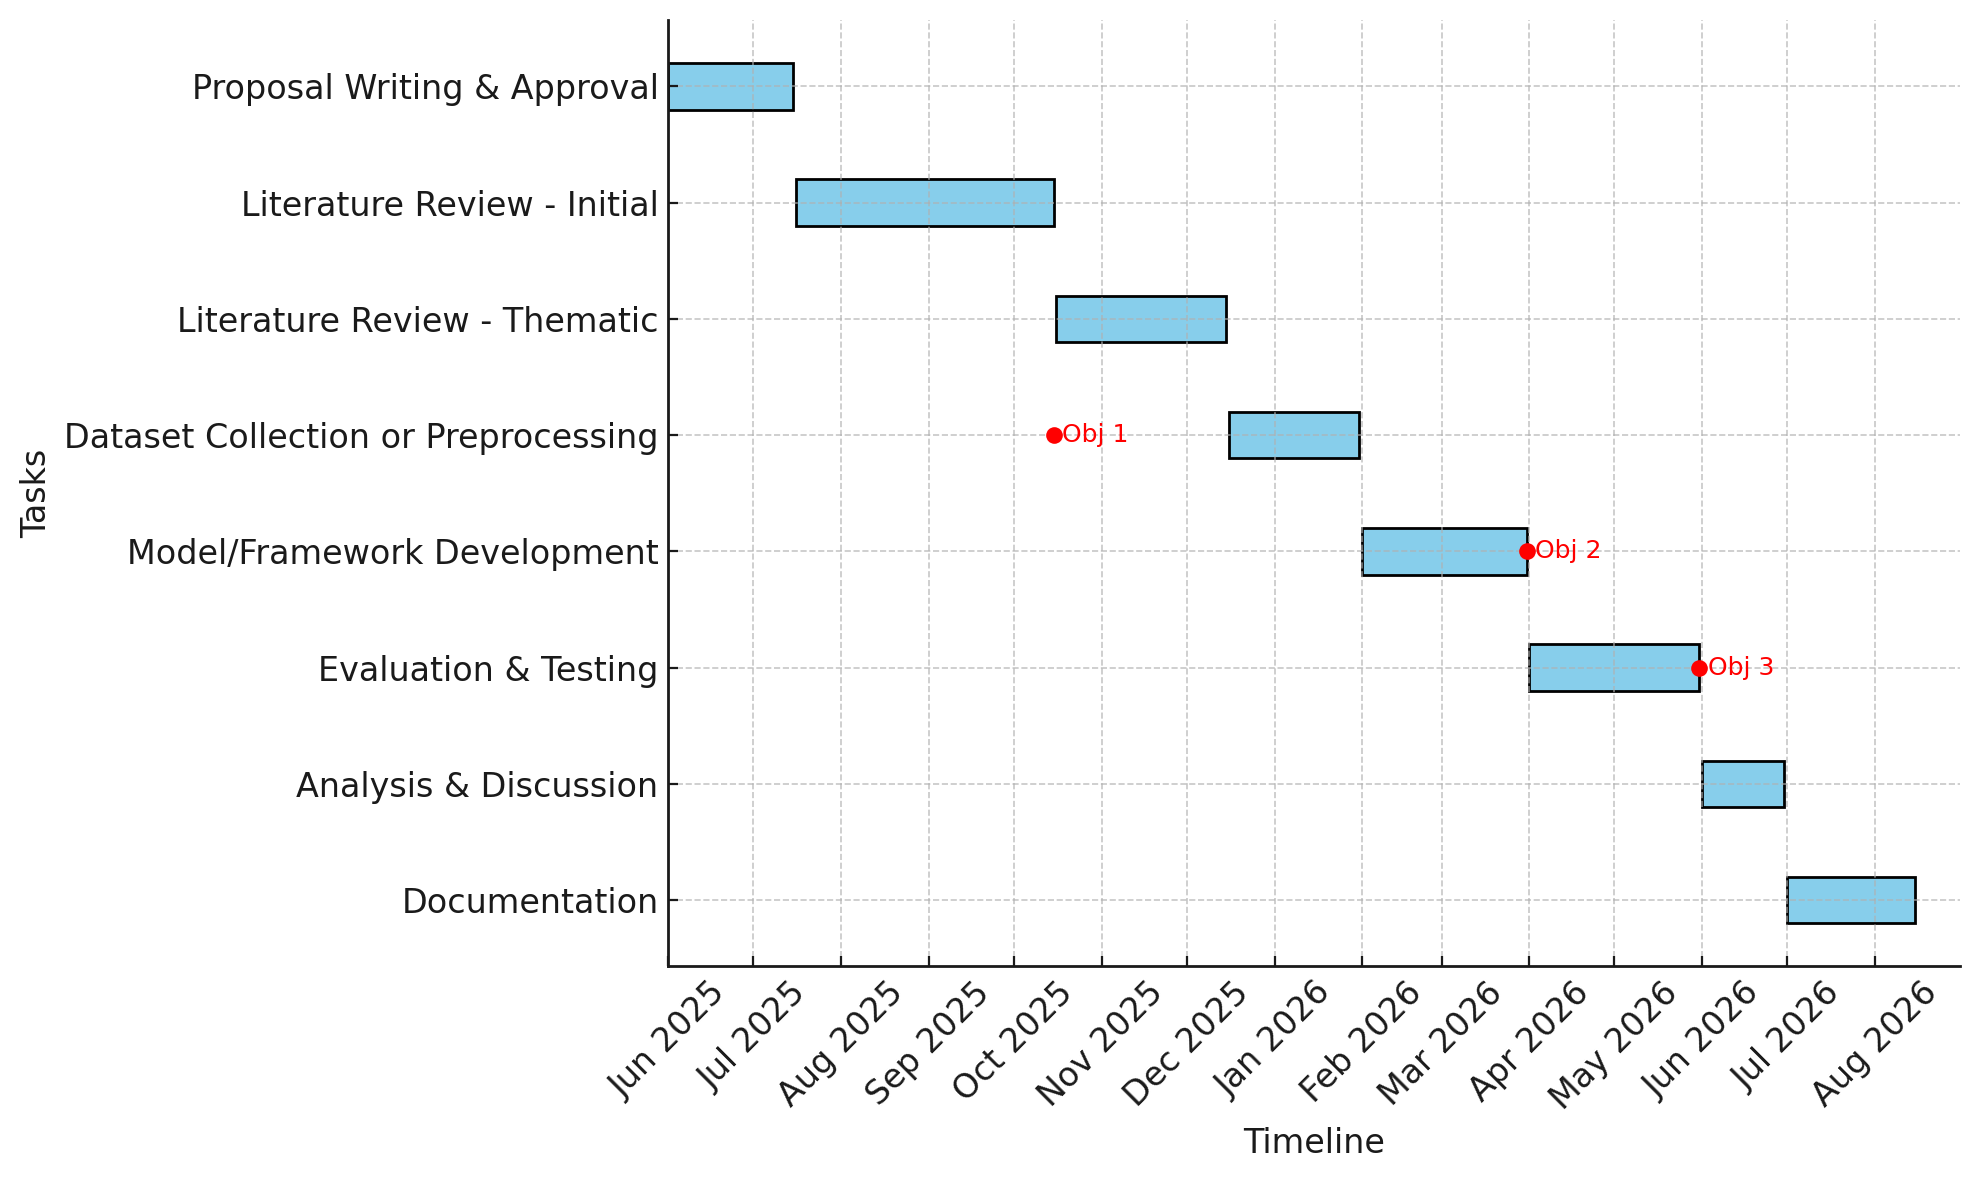
\includegraphics[width=\textwidth]{gantt_chart.png}
		\caption{Project Plan}
	\end{figure}
	